\documentclass[10pt,a4paper]{article}

% ==============================================================================
% PDF 3: PRINTABLE ATTACHMENTS (DIAGRAMS, SCHEMATICS, PHOTOS & CODE BOOKLET)
% Formatted for direct physical A4 printing and notebook pasting
% - 1.0 inch (2.54 cm) Left and Right Margins for perfect trimming/pasting
% - ZERO headers, footers, or page numbers (\pagestyle{empty})
% - NO paste-in instructions boxes inside this printable booklet
% - Generous text line spacing, padding, and enlarged legible diagrams
% - Exactly 6 Self-Contained A4 Pages
% ==============================================================================
\usepackage[utf8]{inputenc}
\usepackage[T1]{fontenc}
\usepackage{lmodern}
\usepackage[left=1.0in, right=1.0in, top=1.1cm, bottom=1.1cm]{geometry}
\usepackage{setspace}
\setstretch{1.10} % Enhanced text readability and line spacing
\usepackage{amsmath,amssymb,amsfonts}
\usepackage{graphicx}
\usepackage{listings}
\usepackage{tikz}
\usepackage{circuitikz}
\usetikzlibrary{shapes.geometric,arrows.meta,positioning,calc}
\usepackage{booktabs}
\usepackage{tabularx}
\usepackage{enumitem}
\usepackage{titlesec}
\usepackage{caption}
\captionsetup{labelformat=empty, font=small, labelfont=bf, justification=centering, skip=5pt}
\usepackage{microtype}
\usepackage{float}

% Strict No Header / No Footer / No Page Numbers
\pagestyle{empty}

% Typographic Section Formatting with balanced spacing
\titleformat{\section}
  {\normalfont\large\bfseries}{\thesection}{1em}{}[\titlerule]
\titleformat{\subsection}
  {\normalfont\normalsize\bfseries}{\thesubsection}{0.8em}{}

\titlespacing*{\section}{0pt}{4pt}{3pt}
\titlespacing*{\subsection}{0pt}{4pt}{2pt}

% Listings Styling (Strict Monochrome, Clear Readable Font with Generous Spacing)
\lstdefinestyle{bwArduinoPrintLarge}{
    language=C++,
    basicstyle=\ttfamily\small,
    keywordstyle=\bfseries,
    commentstyle=\itshape,
    stringstyle=\ttfamily,
    numbers=left,
    numberstyle=\footnotesize,
    numbersep=6pt,
    stepnumber=1,
    breaklines=true,
    breakatwhitespace=true,
    frame=single,
    rulecolor=\color{black},
    tabsize=2,
    showstringspaces=false,
    columns=fullflexible,
    keepspaces=true,
    lineskip=1.2pt,
    aboveskip=4pt,
    belowskip=4pt
}

\lstdefinestyle{bwTerminalPrintLarge}{
    basicstyle=\ttfamily\small,
    numbers=none,
    breaklines=true,
    breakatwhitespace=true,
    frame=single,
    rulecolor=\color{black},
    columns=fullflexible,
    keepspaces=true,
    lineskip=1.5pt,
    aboveskip=4pt,
    belowskip=4pt
}

\setlength{\tabcolsep}{6pt}

\begin{document}

% ==============================================================================
% SHEET 1 (PAGE 1): EXPERIMENT 01 - IOT ARCHITECTURE & PROTOCOL MODELS
% ==============================================================================
\section*{Experiment 01: Overview of IoT Architecture \& Protocols}

\subsection*{1. 5-Tier Hierarchical IoT Architecture Reference Framework}
\begin{figure}[H]
\centering
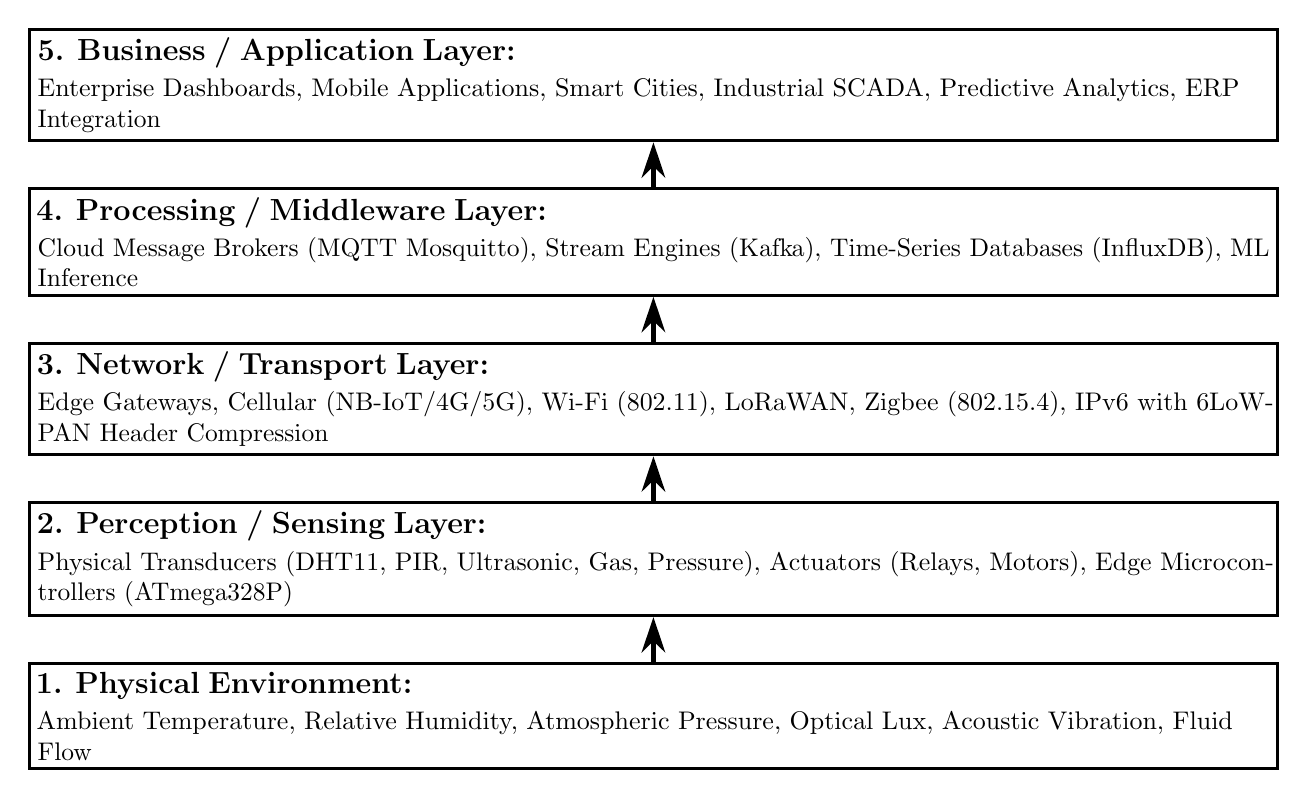
\begin{tikzpicture}[scale=0.92, every node/.style={transform shape}]
    \tikzstyle{layer} = [rectangle, draw=black, fill=white, line width=1.1pt, text width=17.0cm, minimum height=1.45cm, font=\normalsize, align=left]
    \tikzstyle{arr} = [ultra thick, -{Stealth[length=4.5mm, width=3.0mm]}, draw=black]

    \node [layer] (l5) {\textbf{\large 5. Business / Application Layer:}\\[0.08cm] Enterprise Dashboards, Mobile Applications, Smart Cities, Industrial SCADA, Predictive Analytics, ERP Integration};
    \node [layer, below=0.62cm of l5] (l4) {\textbf{\large 4. Processing / Middleware Layer:}\\[0.08cm] Cloud Message Brokers (MQTT Mosquitto), Stream Engines (Kafka), Time-Series Databases (InfluxDB), ML Inference};
    \node [layer, below=0.62cm of l4] (l3) {\textbf{\large 3. Network / Transport Layer:}\\[0.08cm] Edge Gateways, Cellular (NB-IoT/4G/5G), Wi-Fi (802.11), LoRaWAN, Zigbee (802.15.4), IPv6 with 6LoWPAN Header Compression};
    \node [layer, below=0.62cm of l3] (l2) {\textbf{\large 2. Perception / Sensing Layer:}\\[0.08cm] Physical Transducers (DHT11, PIR, Ultrasonic, Gas, Pressure), Actuators (Relays, Motors), Edge Microcontrollers (ATmega328P)};
    \node [layer, below=0.62cm of l2] (l1) {\textbf{\large 1. Physical Environment:}\\[0.08cm] Ambient Temperature, Relative Humidity, Atmospheric Pressure, Optical Lux, Acoustic Vibration, Fluid Flow};

    \draw [arr] (l1.north) -- (l2.south);
    \draw [arr] (l2.north) -- (l3.south);
    \draw [arr] (l3.north) -- (l4.south);
    \draw [arr] (l4.north) -- (l5.south);
\end{tikzpicture}
\caption{\textbf{Figure 1.1: 5-Tier Hierarchical IoT Architecture Reference Framework.}}
\end{figure}

\vspace{0.35cm}
\subsection*{2. Constrained IoT Communication Protocols Comparison}
\begin{table}[H]
\centering
\normalsize
\setlength{\tabcolsep}{4.5pt}
\renewcommand{\arraystretch}{1.50}
\begin{tabularx}{\textwidth}{|p{2.0cm}|p{1.8cm}|p{3.0cm}|p{2.0cm}|X|}
\hline
\textbf{Protocol} & \textbf{Transport} & \textbf{Messaging Model} & \textbf{Header Size} & \textbf{Primary Application Domain} \\
\hline
\textbf{MQTT} & TCP (1883) & Publish / Subscribe & 2 Bytes (Fixed) & Real-time sensor telemetry, SCADA, battery-backed nodes. \\
\textbf{CoAP} & UDP (5683) & REST Request / Response & 4 Bytes (Fixed) & Constrained 8-bit MCUs, low-power lossy networks (LLNs). \\
\textbf{\small HTTP/REST} & TCP (80/443) & Client / Server Request & $>500$ B (Text) & Cloud-to-cloud APIs, enterprise REST integrations. \\
\textbf{WebSocket} & TCP (80) & Full-Duplex Stream & 2--10 Bytes & Live browser telemetry monitoring dashboards. \\
\hline
\end{tabularx}
\caption{\textbf{Table 1.1: Comparison of Constrained Application Protocols in IoT Systems.}}
\end{table}

\newpage

% ==============================================================================
% SHEET 2 (PAGE 2): EXPERIMENT 02 - HARDWARE LAYOUT & SCHEMATICS (ENLARGED & STACKED)
% ==============================================================================
\section*{Experiment 02: Hardware Configuration \& Interfacing Schematics}

\subsection*{1. Arduino UNO R3 Hardware Architecture \& Pinout}
\begin{figure}[H]
\centering
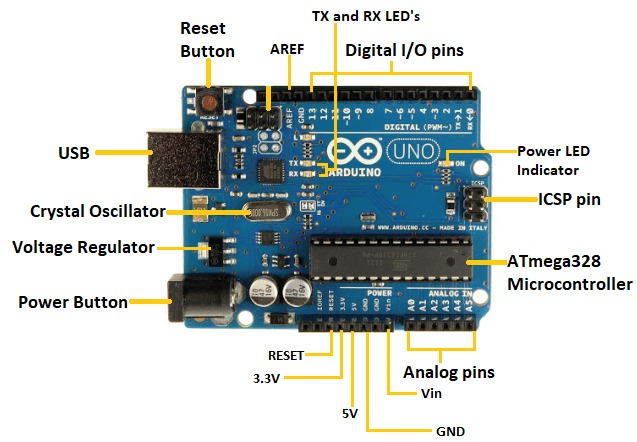
\includegraphics[width=0.62\textwidth]{Arduino Board Configuration.jpg}
\caption{\textbf{Figure 2.1: Arduino UNO R3 Hardware Architecture and Pin Configuration Layout.}}
\end{figure}

\vspace{-0.3cm}
\subsection*{2. Dual Alternating LED Interfacing Layouts}
\begin{figure}[H]
\centering
% Stacked Up: Breadboard Fritzing Wiring (Enlarged)
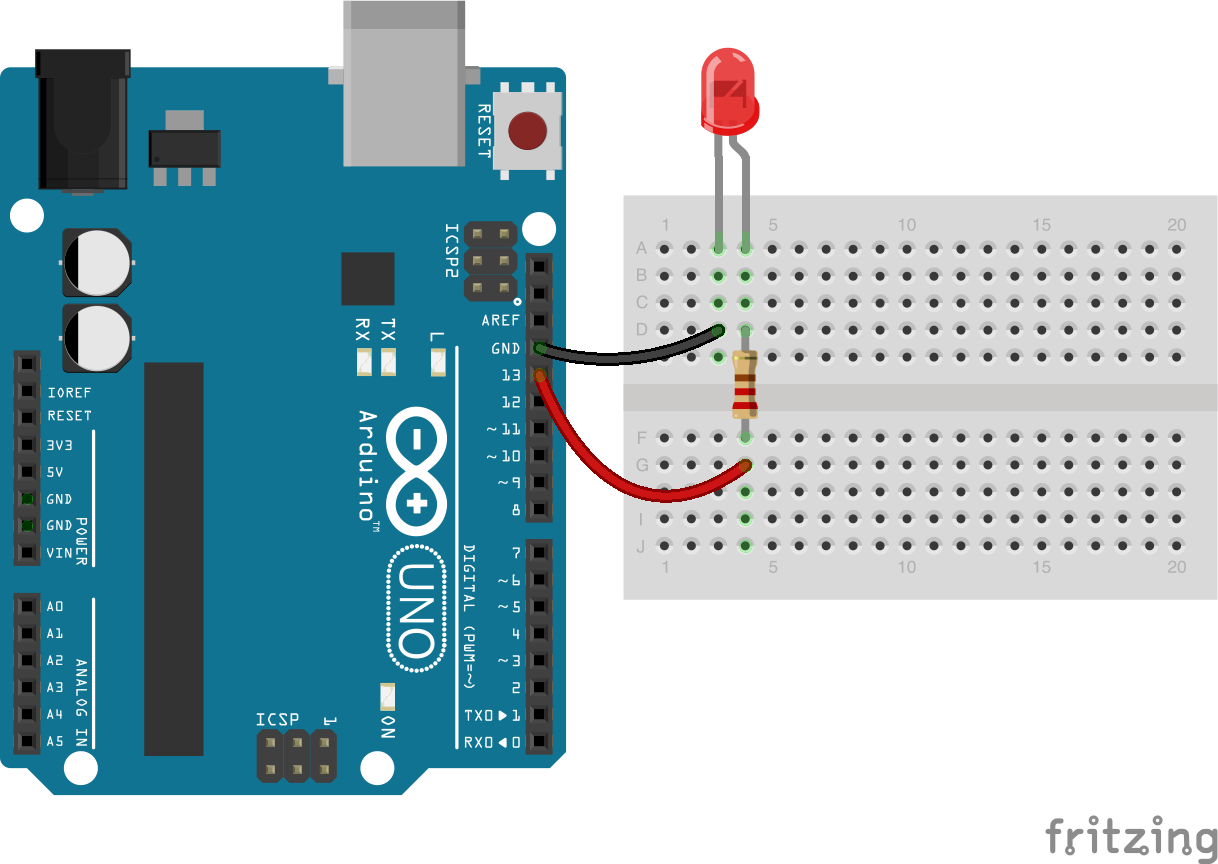
\includegraphics[height=3.8cm, keepaspectratio]{led_resistor.png}
\caption{\textbf{Figure 2.2: Breadboard Fritzing Wiring Layout for Dual LED Interfacing.}}
\end{figure}

\vspace{-0.35cm}
\begin{figure}[H]
\centering
% Stacked Down: CircuiTikZ Dual-LED Schematic (Enlarged & Wide)
\begin{circuitikz}[american, scale=0.74]
    \draw[fill=white, draw=black, line width=1.0pt] (0,0) rectangle (4.2,3.8);
    \node at (2.1,3.3) [font=\bfseries\small] {ARDUINO UNO};
    
    \node (p8) at (4.2,2.6) [anchor=east, font=\small\bfseries] {D8 (Pin 8)};
    \node (p7) at (4.2,1.5) [anchor=east, font=\small\bfseries] {D7 (Pin 7)};
    \node (gnd) at (4.2,0.5) [anchor=east, font=\small\bfseries] {GND};

    \draw (4.2,2.6) -- (5.2,2.6) to[R, l=$R_1(1\,\text{k}\Omega)$, *-] (7.2,2.6) to[leDo, -*] (9.2,2.6) -- (9.2,0.5);
    \node[right, font=\small\bfseries] at (9.3,2.6) {$\text{LED}_1\ (\text{Green})$};

    \draw (4.2,1.5) -- (5.2,1.5) to[R, l=$R_2(1\,\text{k}\Omega)$, *-] (7.2,1.5) to[leDo, -*] (9.2,1.5) -- (9.2,0.5);
    \node[right, font=\small\bfseries] at (9.3,1.5) {$\text{LED}_2\ (\text{Red})$};

    \draw (4.2,0.5) -- (9.2,0.5) node[ground]{};
\end{circuitikz}
\caption{\textbf{Figure 2.3: CircuiTikZ Dual-LED Interfacing Circuit Schematic.}}
\end{figure}

\vspace{-0.35cm}
\subsection*{3. Hardware Pin Wiring Interconnection Matrix}
\begin{table}[H]
\centering
\small
\renewcommand{\arraystretch}{1.22}
\begin{tabularx}{\textwidth}{|l|l|l|X|}
\hline
\textbf{Arduino Terminal} & \textbf{Breadboard Component} & \textbf{Component Terminal} & \textbf{Signal Function} \\
\hline
Digital Pin 8 (D8) & Resistor $R_1$ ($1\,\text{k}\Omega$) & Lead 1 & GPIO Push-Pull Output Channel 1 \\
Resistor $R_1$ ($1\,\text{k}\Omega$) & $\text{LED}_1$ (Green) & Anode (Long Leg, $+$) & Current-Limited 5V Drive ($I_{F1} \approx 3.0\text{ mA}$) \\
$\text{LED}_1$ (Green) & Common Ground Rail & Cathode (Flat Notch, $-$) & System Ground Return Path \\
\hline
Digital Pin 7 (D7) & Resistor $R_2$ ($1\,\text{k}\Omega$) & Lead 1 & GPIO Push-Pull Output Channel 2 \\
Resistor $R_2$ ($1\,\text{k}\Omega$) & $\text{LED}_2$ (Red) & Anode (Long Leg, $+$) & Current-Limited 5V Drive ($I_{F2} \approx 3.0\text{ mA}$) \\
$\text{LED}_2$ (Red) & Common Ground Rail & Cathode (Flat Notch, $-$) & System Ground Return Path \\
\hline
\end{tabularx}
\caption{\textbf{Table 2.1: Pin Wiring Interconnection Matrix for Experiment 2.}}
\end{table}

\newpage

% ==============================================================================
% SHEET 3 (PAGE 3): EXPERIMENT 02 - SOURCE CODE, WAVEFORMS & TRUTH TABLE
% ==============================================================================
\section*{Experiment 02: Firmware Code, Waveforms \& Truth Table}

\subsection*{1. Complete Arduino C++ Firmware Code}
\begin{lstlisting}[style=bwArduinoPrintLarge, title={\textbf{Program Listing 2.1: Complete Arduino C++ Program for Dual Alternating LED Blinking}}]
/*
 * Experiment 02: Dual Alternating LED Interfacing with Arduino UNO
 * Hardware Pin Connections: Pin D8 -> Green LED | Pin D7 -> Red LED
 * Switching Interval: 1000 ms (1.0 second) Anti-Phase Blinking
 */

const int LED1_PIN = 8;    // Green LED Channel (Digital Pin 8)
const int LED2_PIN = 7;    // Red LED Channel (Digital Pin 7)
const unsigned long BLINK_INTERVAL = 1000; // Period: 1000 ms (1.0 s)

void setup() {
  // Configure both GPIO pins as digital output drivers
  pinMode(LED1_PIN, OUTPUT);
  pinMode(LED2_PIN, OUTPUT);
  
  // Set deterministic initial state (both OFF)
  digitalWrite(LED1_PIN, LOW);
  digitalWrite(LED2_PIN, LOW);
}

void loop() {
  // Phase 1: LED1 ON (Active HIGH), LED2 OFF (Active LOW)
  digitalWrite(LED1_PIN, HIGH);
  digitalWrite(LED2_PIN, LOW);
  delay(BLINK_INTERVAL);
  
  // Phase 2: LED1 OFF (Active LOW), LED2 ON (Active HIGH)
  digitalWrite(LED1_PIN, LOW);
  digitalWrite(LED2_PIN, HIGH);
  delay(BLINK_INTERVAL);
}
\end{lstlisting}

\vspace{0.1cm}
\subsection*{2. Logic State Transitions \& Timing Waveforms}
\begin{figure}[H]
\centering
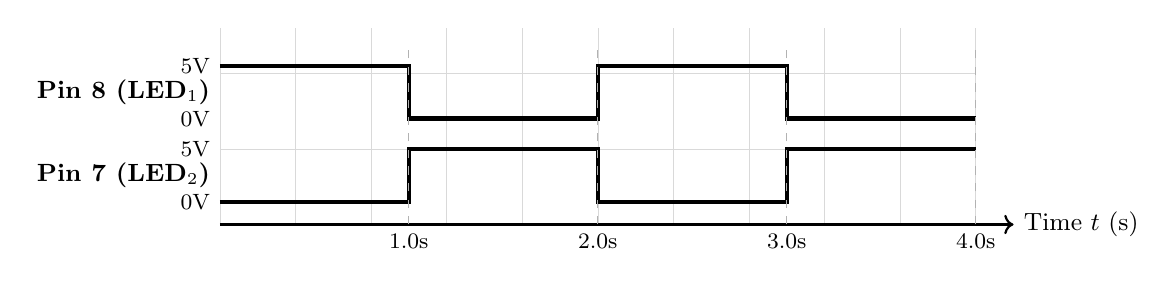
\begin{tikzpicture}[scale=0.96]
    \draw[step=1.0cm,gray!30,very thin] (0,0) grid (10,2.6);
    \draw[thick,->] (0,0) -- (10.5,0) node[right, font=\small] {Time $t$ (s)};
    
    % Pin 8 (LED1)
    \draw[ultra thick] (0,2.1) -- (2.5,2.1) -- (2.5,1.4) -- (5.0,1.4) -- (5.0,2.1) -- (7.5,2.1) -- (7.5,1.4) -- (10.0,1.4);
    \node[left, font=\small\bfseries] at (0,1.75) {Pin 8 ($\text{LED}_1$)};
    \node[left, font=\footnotesize] at (0,2.1) {5V};
    \node[left, font=\footnotesize] at (0,1.4) {0V};

    % Pin 7 (LED2)
    \draw[ultra thick] (0,0.3) -- (2.5,0.3) -- (2.5,1.0) -- (5.0,1.0) -- (5.0,0.3) -- (7.5,0.3) -- (7.5,1.0) -- (10.0,1.0);
    \node[left, font=\small\bfseries] at (0,0.65) {Pin 7 ($\text{LED}_2$)};
    \node[left, font=\footnotesize] at (0,1.0) {5V};
    \node[left, font=\footnotesize] at (0,0.3) {0V};
    
    \foreach \x/\t in {2.5/1.0s, 5.0/2.0s, 7.5/3.0s, 10.0/4.0s} {
        \draw[dashed, gray!60] (\x,0) -- (\x,2.4);
        \node[below, font=\footnotesize] at (\x,0) {\t};
    }
\end{tikzpicture}
\caption{\textbf{Figure 2.4: Digital Logic Timing Waveforms for Anti-Phase Switching ($T = 1.0\,\text{s}$).}}
\end{figure}

\vspace{-0.1cm}
\subsection*{3. Circuit Logic Truth Table}
\begin{table}[H]
\centering
\small
\renewcommand{\arraystretch}{1.32}
\begin{tabularx}{\textwidth}{|c|c|c|c|c|X|}
\hline
\textbf{Time Interval} & \textbf{Pin 8 Level} & \textbf{Pin 7 Level} & \textbf{$\text{LED}_1$ State} & \textbf{$\text{LED}_2$ State} & \textbf{Circuit Current \& Physical Observation} \\
\hline
$0.0\,\text{s} - 1.0\,\text{s}$ & HIGH ($5.0\,\text{V}$) & LOW ($0.0\,\text{V}$) & \textbf{ON} & \textbf{OFF} & $I_{F1} \approx 3.0\text{ mA}$; Green light emission active. \\
$1.0\,\text{s} - 2.0\,\text{s}$ & LOW ($0.0\,\text{V}$) & HIGH ($5.0\,\text{V}$) & \textbf{OFF} & \textbf{ON} & $I_{F2} \approx 3.0\text{ mA}$; Red light emission active. \\
$2.0\,\text{s} - 3.0\,\text{s}$ & HIGH ($5.0\,\text{V}$) & LOW ($0.0\,\text{V}$) & \textbf{ON} & \textbf{OFF} & State repeats in strict periodic anti-phase. \\
\hline
\end{tabularx}
\caption{\textbf{Table 2.2: Truth Table and Circuit State Sequence.}}
\end{table}

\newpage

% ==============================================================================
% SHEET 4 (PAGE 4): EXPERIMENT 03 - SENSOR PROTOCOLS & SCHEMATICS (ENLARGED & STACKED)
% ==============================================================================
\section*{Experiment 03: DHT11 Sensor Protocols \& Circuit Schematics}

\subsection*{1. DHT11 Single-Bus (1-Wire) Communication Handshake}
\begin{figure}[H]
\centering
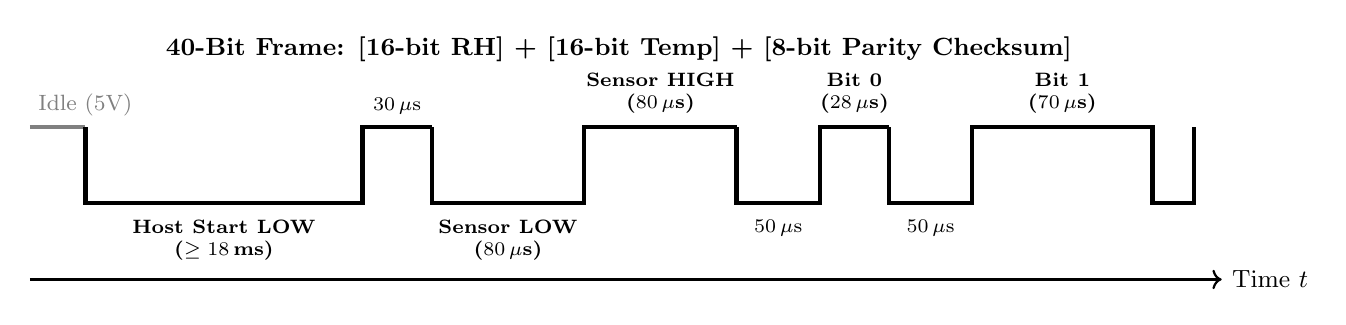
\begin{tikzpicture}[scale=0.88]
    \draw[thick, ->] (0,-0.4) -- (17.2,-0.4) node[right, font=\small] {Time $t$};
    
    % Idle State
    \draw[ultra thick, gray] (0,1.8) -- (0.8,1.8) node[above, font=\footnotesize] {Idle (5V)};
    
    % Host Start Signal (LOW >= 18ms, then HIGH 20-40us)
    \draw[ultra thick] (0.8,1.8) -- (0.8,0.7) -- (4.8,0.7) -- (4.8,1.8) -- (5.8,1.8);
    \node[below, font=\scriptsize\bfseries, align=center] at (2.8,0.6) {Host Start LOW\\($\ge 18\,\text{ms}$)};
    \node[above, font=\scriptsize] at (5.3,1.85) {$30\,\mu\text{s}$};
    
    % Sensor Response (LOW 80us, then HIGH 80us)
    \draw[ultra thick] (5.8,1.8) -- (5.8,0.7) -- (8.0,0.7) -- (8.0,1.8) -- (10.2,1.8);
    \node[below, font=\scriptsize\bfseries, align=center] at (6.9,0.6) {Sensor LOW\\($80\,\mu\text{s}$)};
    \node[above, font=\scriptsize\bfseries, align=center] at (9.1,1.85) {Sensor HIGH\\($80\,\mu\text{s}$)};
    
    % Bit 0 (LOW 50us, HIGH 28us)
    \draw[ultra thick] (10.2,1.8) -- (10.2,0.7) -- (11.4,0.7) -- (11.4,1.8) -- (12.4,1.8);
    \node[below, font=\scriptsize] at (10.8,0.6) {$50\,\mu\text{s}$};
    \node[above, font=\scriptsize\bfseries, align=center] at (11.9,1.85) {Bit 0\\($28\,\mu\text{s}$)};
    
    % Bit 1 (LOW 50us, HIGH 70us)
    \draw[ultra thick] (12.4,1.8) -- (12.4,0.7) -- (13.6,0.7) -- (13.6,1.8) -- (16.2,1.8) -- (16.2,0.7) -- (16.8,0.7) -- (16.8,1.8);
    \node[below, font=\scriptsize] at (13.0,0.6) {$50\,\mu\text{s}$};
    \node[above, font=\scriptsize\bfseries, align=center] at (14.9,1.85) {Bit 1\\($70\,\mu\text{s}$)};
    
    \node[above, font=\small\bfseries] at (8.5,2.6) {40-Bit Frame: [16-bit RH] + [16-bit Temp] + [8-bit Parity Checksum]};
\end{tikzpicture}
\caption{\textbf{Figure 3.1: DHT11 Single-Bus 1-Wire Handshake and Bit Timing Sequence.}}
\end{figure}

\vspace{-0.3cm}
\subsection*{2. DHT11 Sensor Breadboard Wiring \& Interfacing Circuit Schematic}
\begin{figure}[H]
\centering
% Stacked Up: DHT11 Breadboard Wiring (Enlarged)
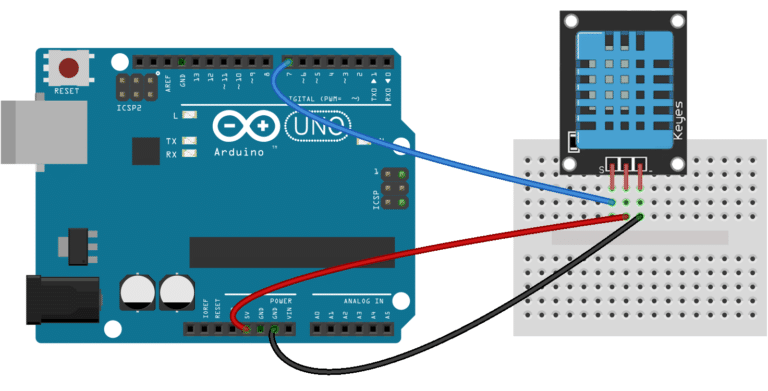
\includegraphics[height=3.8cm, keepaspectratio]{dht11_wiring.png}
\caption{\textbf{Figure 3.2: DHT11 Breadboard Fritzing Wiring Layout.}}
\end{figure}

\vspace{-0.35cm}
\begin{figure}[H]
\centering
% Stacked Down: CircuiTikZ Schematic (Enlarged & Wide)
\begin{circuitikz}[american, scale=0.74]
    \draw[fill=white, draw=black, line width=1.0pt] (0,0) rectangle (4.2,4.0);
    \node at (2.1,3.5) [font=\bfseries\small] {ARDUINO UNO};
    
    \node (p5v) at (4.2,2.9) [anchor=east, font=\small\bfseries] {5V};
    \node (pd7) at (4.2,2.0) [anchor=east, font=\small\bfseries] {D7};
    \node (pd8) at (4.2,1.1) [anchor=east, font=\small\bfseries] {D8};
    \node (pgnd) at (4.2,0.4) [anchor=east, font=\small\bfseries] {GND};

    \draw[fill=white, draw=black, line width=0.9pt] (8.2,1.5) rectangle (11.4,3.9);
    \node at (9.8,3.4) [font=\bfseries\small] {DHT11 MODULE};
    \node (d_vcc) at (8.2,2.9) [anchor=west, font=\small] {VCC (+)};
    \node (d_dat) at (8.2,2.2) [anchor=west, font=\small] {DATA};
    \node (d_gnd) at (8.2,1.7) [anchor=west, font=\small] {GND (-)};

    \draw (4.2,2.9) -- (8.2,2.9);
    \draw (4.2,2.0) -- (8.2,2.2);
    \draw (4.2,0.4) -- (6.0,0.4) -- (6.0,1.4) -- (7.6,1.4) -- (7.6,1.7) -- (8.2,1.7);

    \draw (4.2,1.1) -- (5.0,1.1) to[R, l=$R_{\text{alert}}(220\,\Omega)$, *-] (6.8,1.1) to[leDo, -*] (8.4,1.1) -- (8.4,0.4) -- (4.2,0.4) node[ground]{};
    \node[right, font=\small\bfseries] at (8.5,1.1) {$\text{LED}_{\text{alert}}$};
\end{circuitikz}
\caption{\textbf{Figure 3.3: DHT11 Sensor \& High-Temperature Alert LED Circuit Schematic.}}
\end{figure}

\vspace{-0.35cm}
\subsection*{3. Hardware Pin Wiring Interconnection Matrix}
\begin{table}[H]
\centering
\small
\renewcommand{\arraystretch}{1.22}
\begin{tabularx}{\textwidth}{|l|l|l|X|}
\hline
\textbf{Arduino UNO Pin} & \textbf{External Component} & \textbf{Component Terminal} & \textbf{Functional Role} \\
\hline
$+5\text{V}$ & DHT11 Module & Pin 1 ($V_{CC} / +$) & Sensor DC Power Supply ($+5\text{V}$) \\
Digital Pin 7 (D7) & DHT11 Module & Pin 2 (DATA / OUT) & Bidirectional 1-Wire Telemetry Line \\
GND & DHT11 Module & Pin 3 (GND / -) & Common System Ground ($0\text{V}$) \\
\hline
Digital Pin 8 (D8) & Resistor $R_{\text{alert}}$ ($220\,\Omega$) & Lead 1 & High-Temperature Alert Output Trigger \\
Resistor $R_{\text{alert}}$ & Alert LED (Red) & Anode (Long Leg, $+$) & Current-Limited LED Driver ($I_F \approx 13.6\text{ mA}$) \\
Alert LED & Arduino GND Rail & Cathode (Flat Notch, $-$) & Ground Return Path \\
\hline
\end{tabularx}
\caption{\textbf{Table 3.1: Hardware Wiring Interconnection Matrix for Experiment 3.}}
\end{table}

\newpage

% ==============================================================================
% SHEET 5 (PAGE 5): EXPERIMENT 03 - COMPLETE SOURCE CODE LISTING
% ==============================================================================
\section*{Experiment 03: Complete Arduino C++ Source Code}

\begin{lstlisting}[style=bwArduinoPrintLarge, title={\textbf{Program Listing 3.1: Complete Arduino C++ Program for DHT11 Telemetry and Closed-Loop Alert Actuation}}]
/*
 * Experiment 03: DHT11 Sensor Interfacing with Closed-Loop High-Temp Alert
 * Pin Connections: DHT11 DATA -> Pin 7 | Alert Red LED -> Pin 8
 * Alarm Trigger Threshold: 30.0 deg C (Adjustable setpoint)
 */

#include <DHT.h>

#define DHTPIN 7            // DHT11 DATA connected to Digital Pin 7
#define DHTTYPE DHT11       // Sensor model designation
#define ALERT_PIN 8         // Red Alert LED connected to Digital Pin 8
#define TEMP_THRESHOLD 30.0 // Closed-loop alarm trigger setpoint in Celsius

DHT dht(DHTPIN, DHTTYPE);

void setup() {
  Serial.begin(9600);
  pinMode(ALERT_PIN, OUTPUT);
  digitalWrite(ALERT_PIN, LOW); // Initialize alert LED to OFF
  dht.begin();
  
  Serial.println("=================================================");
  Serial.println("   IoT Lab: DHT11 Telemetry & Alert System       ");
  Serial.println("=================================================");
  Serial.println("Time(s)\tHumidity(%)\tTemp(C)\tAlert Status");
}

void loop() {
  // DHT11 sampling rate is limited to 1 Hz; enforce 2.0 s polling interval
  delay(2000);

  float humidity = dht.readHumidity();
  float temperature = dht.readTemperature();

  // Validate sensor readout
  if (isnan(humidity) || isnan(temperature)) {
    Serial.println("ERROR: Failed to read from DHT11 sensor!");
    return;
  }

  // Closed-Loop Threshold Comparison Logic
  bool isAlert = (temperature >= TEMP_THRESHOLD);
  digitalWrite(ALERT_PIN, isAlert ? HIGH : LOW);

  // Stream formatted telemetry to Serial Monitor
  Serial.print(millis() / 1000);
  Serial.print(" s\t");
  Serial.print(humidity, 1);
  Serial.print(" %\t\t");
  Serial.print(temperature, 1);
  Serial.print(" C\t");
  Serial.println(isAlert ? "ACTIVE [ALERT ON]" : "NORMAL [OFF]");
}
\end{lstlisting}

\newpage

% ==============================================================================
% SHEET 6 (PAGE 6): EXPERIMENT 03 - OBSERVATIONS & SERIAL TERMINAL STREAM
% ==============================================================================
\section*{Experiment 03: Telemetry Observations \& Serial Output}

\subsection*{1. Experimental Telemetry Observations \& Checksum Verification}
\begin{table}[H]
\centering
\small
\renewcommand{\arraystretch}{1.38}
\begin{tabularx}{\textwidth}{|c|p{3.2cm}|c|c|c|X|}
\hline
\textbf{S.No} & \textbf{Thermal State} & \textbf{Temp} & \textbf{Humidity} & \textbf{Alert Status ($T \ge 30^\circ\text{C}$)} & \textbf{Checksum Parity Calculation} \\
\hline
1 & Ambient Lab Environment & $27.4^\circ\text{C}$ & $62.0\%$ & \textbf{OFF (Normal)} & $\text{0x1B} + \text{0x00} + \text{0x3E} + \text{0x00} = \text{0x59}$ [PASS] \\
2 & Ambient Lab Environment & $28.1^\circ\text{C}$ & $60.5\%$ & \textbf{OFF (Normal)} & $\text{0x1C} + \text{0x00} + \text{0x3C} + \text{0x00} = \text{0x58}$ [PASS] \\
3 & Elevated Heat Applied & $31.8^\circ\text{C}$ & $74.0\%$ & \textbf{ON (ACTIVE ALERT)} & $\text{0x1F} + \text{0x00} + \text{0x4A} + \text{0x00} = \text{0x69}$ [PASS] \\
4 & Peak Heated State & $34.0^\circ\text{C}$ & $86.0\%$ & \textbf{ON (ACTIVE ALERT)} & $\text{0x22} + \text{0x00} + \text{0x56} + \text{0x00} = \text{0x78}$ [PASS] \\
5 & Post-Cooling Normal & $28.5^\circ\text{C}$ & $65.0\%$ & \textbf{OFF (Normal)} & $\text{0x1C} + \text{0x00} + \text{0x41} + \text{0x00} = \text{0x5D}$ [PASS] \\
\hline
\end{tabularx}
\caption{\textbf{Table 3.2: Measured Environmental Telemetry and Closed-Loop Alert Evaluation Log.}}
\end{table}

\vspace{0.2cm}
\subsection*{2. Raw Serial Monitor Terminal Output (9600 Baud)}
\begin{lstlisting}[style=bwTerminalPrintLarge, title={\textbf{Serial Monitor Terminal Capture: Raw Telemetry Stream (9600 Baud)}}]
=================================================
   IoT Lab: DHT11 Telemetry & Alert System       
=================================================
Time(s)	Humidity(%)	Temp(C)	Alert Status
2 s	62.0 %		27.4 C	NORMAL [OFF]
4 s	60.5 %		28.1 C	NORMAL [OFF]
6 s	74.0 %		31.8 C	ACTIVE [ALERT ON]  <-- [Thermal Stimulus Applied]
8 s	86.0 %		34.0 C	ACTIVE [ALERT ON]  <-- [Peak Heating Condition]
10 s	65.0 %		28.5 C	NORMAL [OFF]       <-- [Normalized Below 30 C]
\end{lstlisting}

\end{document}
